\section{Tissues Microanatomy and Tumor Evidences} \label{ssec:micr_anat}


\subsection{Pancreas Microanatomy} \label{ssec:pancr_anat}
    The Pancreas is an internal organ of the human body, part of both the digestive system and the endocrine system. It acts as a gland with both endocrine and exocrine functions, and it is located in the abdomen behind the stomach. Its main endocrine duty is the secretion of hormones like insulin and glucagon which are responsable for the regulation of sugar levels in the blood. As a part of the digestive system instead it acts as an exocrine gland secreting pancreatic juice. The majority of pancreatic tissue has a digestive role, and the cells with this role form clusters (\textit{acini}) around the small pancreatic ducts. The acinus secrete inactive digestive enzymes called zymogens into the small intercalated ducts which they surround, and then in the pancreatic blood vessels system \cite{Pancreas}. In Figure \ref{fig:panc_struct} is shown a picture of the pancreas, with its structure and its placement in the human body.

     \begin{figure}
         \centering
         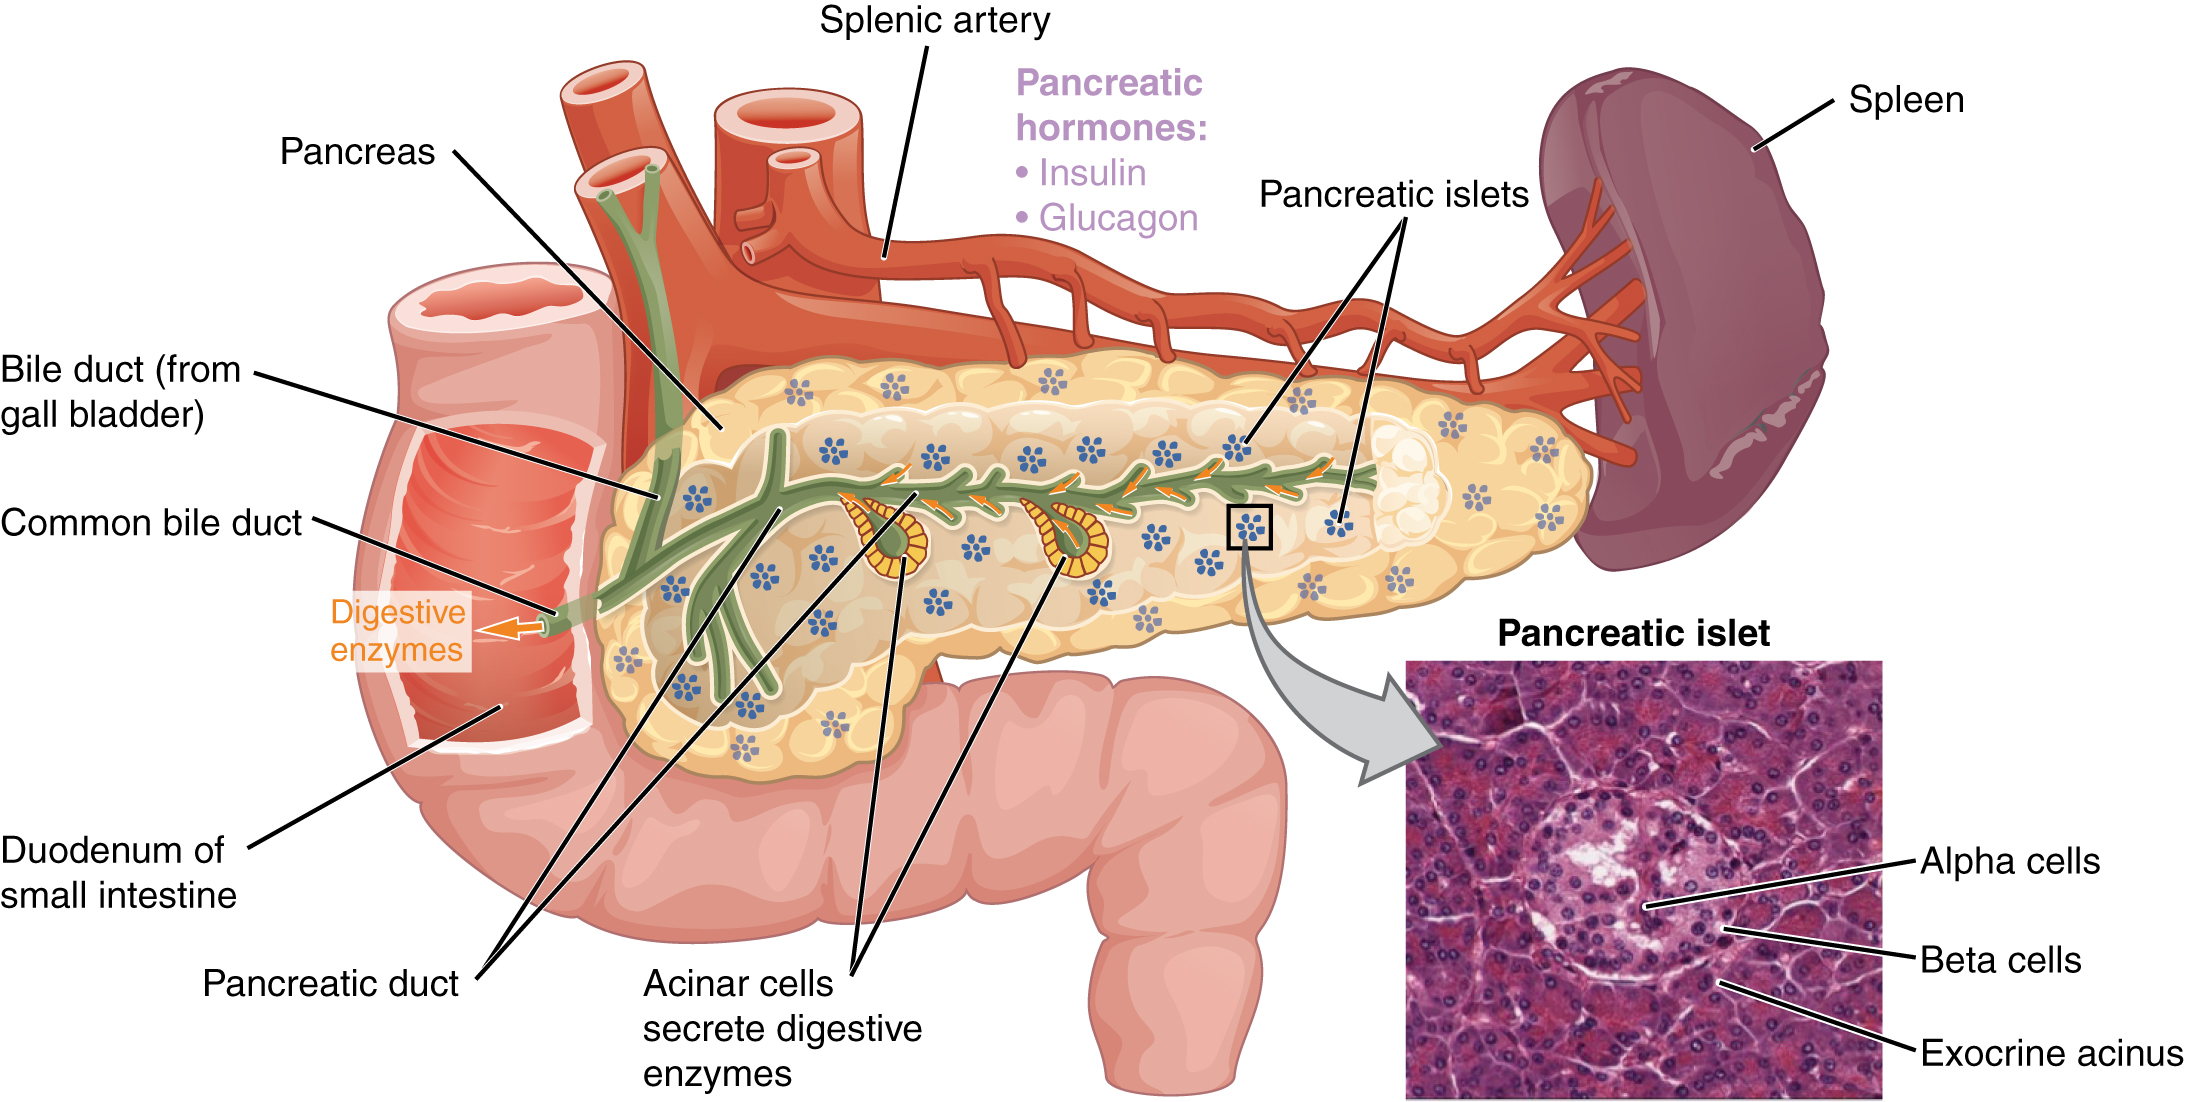
\includegraphics[width = 0.45\textwidth]{images/panc_struct}
         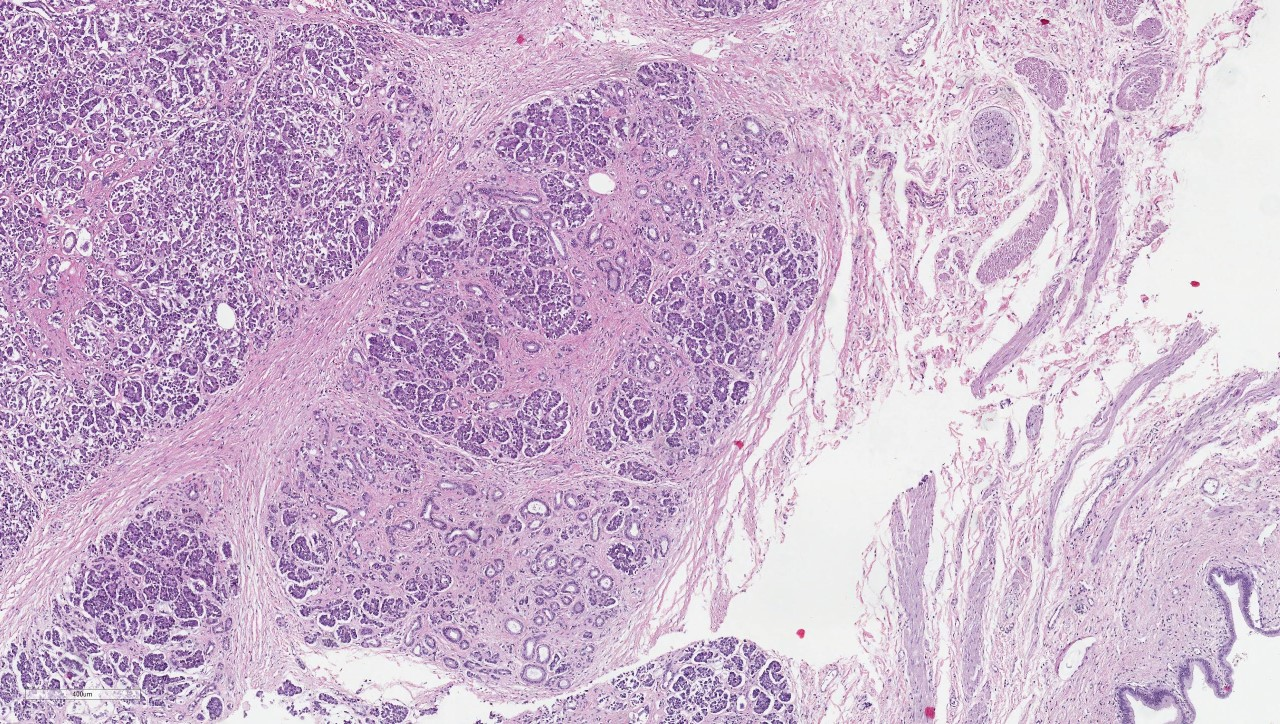
\includegraphics[width = 0.45\textwidth]{images/panc_specimen}
         \caption{(left) A picture of pancreas' structure in its phisiologiacl context. In this picture is clearly visible the macroscopic structure and the galndular organization at microscopic level, and how it reflects in the histological sample. (right) A real pancreatic tissue sample with H\&E staining.}
         \label{fig:panc_struct}
     \end{figure}

    All the tissue is actually rich in other important elements as the islets of Langerhans, and sporadic connective tissue all over the structure, which are clearly visible in the traditional histological specimens.

\subsection{Skin Microanatomy} \label{ssec:derm_anat}
    Skin is the layer of soft, flexible outer tissue covering the body of a vertebrate animal, with the three main functions of protection, regulation, and sensation. Mammalian skin is composed of two primary layers: the epidermis, which provides waterproofing and serves as a barrier to infection, and the dermis, which serves as a location for the appendages of skin. The epidermis is composed of the outermost layers of the skin. It forms a protective barrier over the body's surface, responsible for keeping water in the body and preventing pathogens from entering, and is a stratified squamous epithelium, composed of proliferating basal and differentiated suprabasal keratinocytes. The dermis is the layer of skin beneath the epidermis that consists of connective tissue and cushions the body from stress and strain. The dermis provides tensile strength and elasticity to the skin through an extracellular matrix composed of collagen fibrils, microfibrils, and elastic fibers, embedded in hyaluronan and proteoglycans.

    \begin{figure}
        \centering
        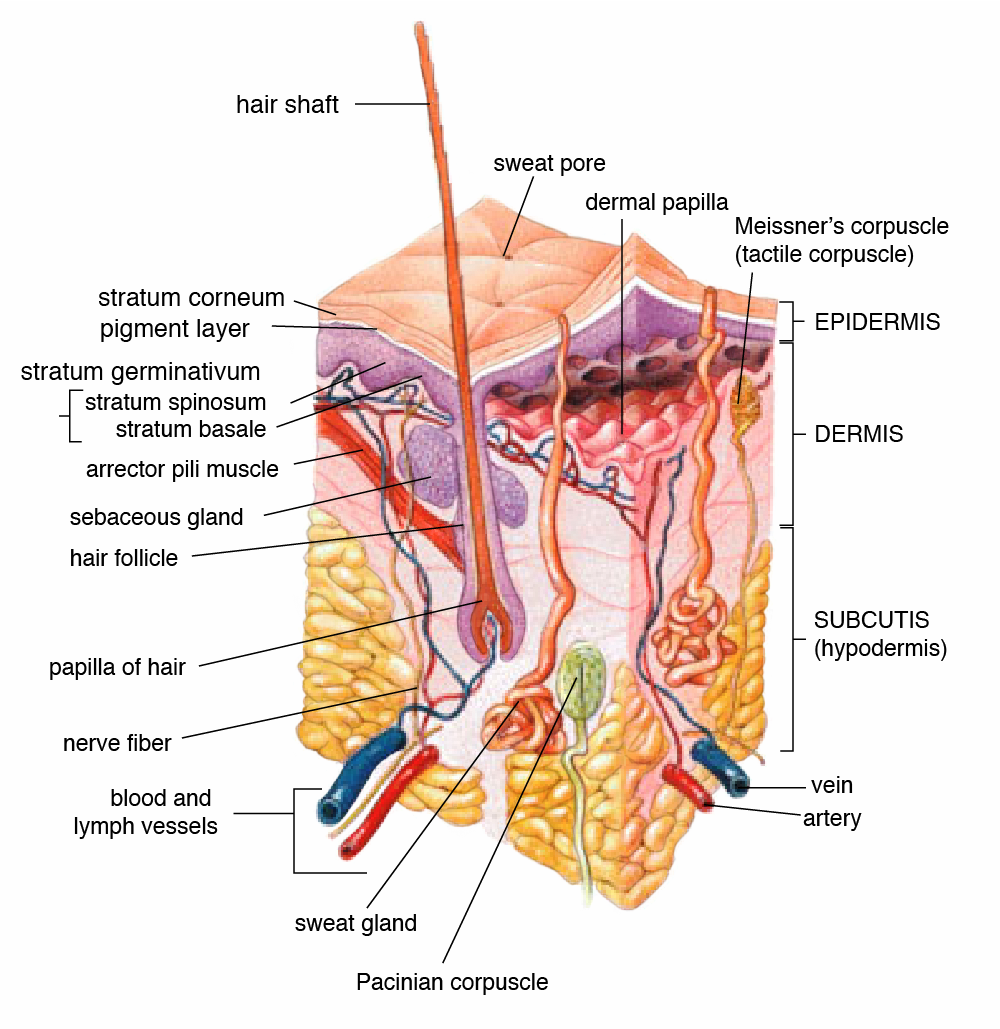
\includegraphics[width = 0.45\textwidth]{images/derm_scheme}
        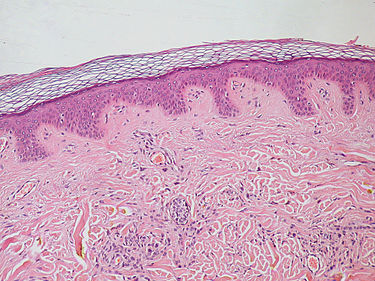
\includegraphics[width = 0.45\textwidth]{images/derm_specimen}

        % \begin{subfigure}[b]{0.45\textwidth}
        %      \centering
        %      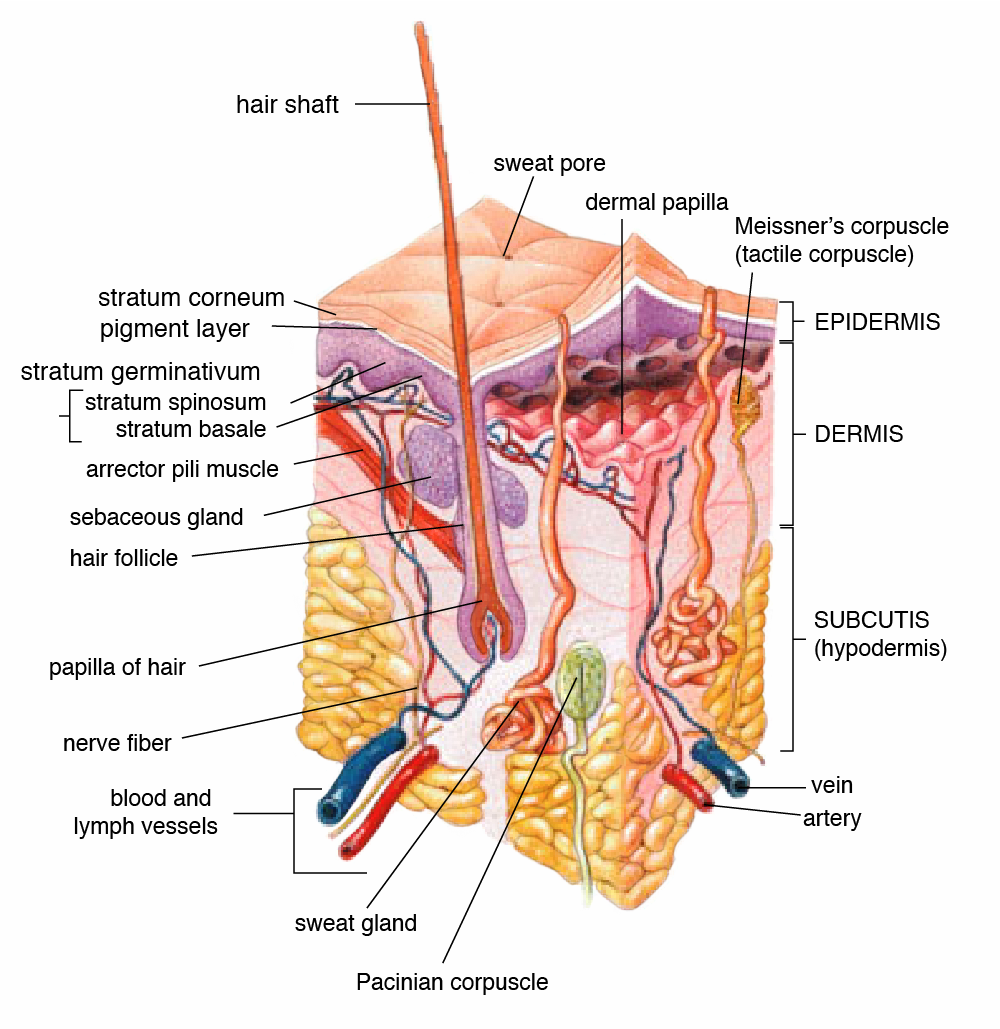
\includegraphics[width = \textwidth]{images/derm_scheme}
        %      \caption{}
        %      \label{fig:derm_scheme}
        % \end{subfigure}
        % \hfill
        % \begin{subfigure}[b]{0.45\textwidth}
        %      \centering
        %      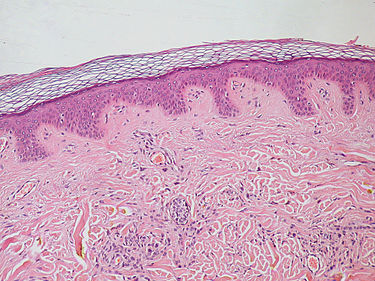
\includegraphics[width = \textwidth]{images/derm_specimen}
        %      \caption{}
        %      \label{fig:derm_specimen}
        % \end{subfigure}
        \caption{(left) Microanatomical description of a region of dermal tissue and all the interesting elements present in cutis, and subcutaneous layer. (right) An actual histological specimen from a sample of dermal tissue.}
        \label{fig:derm_descr}
    \end{figure}

20c2734
